% %% %%%%%%%%%%%%%%%%%%%%%%%%%%%%%%%%%%%%%%%%%%%%%%%%%%%%%%%%%%
% step-1.tex
%
% Author:  Mauricio Matamoros
% License: MIT
%
% %% %%%%%%%%%%%%%%%%%%%%%%%%%%%%%%%%%%%%%%%%%%%%%%%%%%%%%%%%%%

%!TEX root = ../practica.tex
%!TEX root = ../references.bib

% CHKTEX-FILE 1
% CHKTEX-FILE 13
% CHKTEX-FILE 46

\subsection{Paso 1: Alambrado}%
\label{sec:step1}
\begin{importantbox}{\large Importante}
	\begin{center}
		Aunque el RP2040 cuenta con un regulador de 5V integrado, opera a 3.3V. Asegúrese de conectar \VCC únicamente a V\textsubscript{\textsc{bus}} (Pin 38) para no quemarlo.
	\end{center}
\end{importantbox}
\medskip


El proceso de alambrado de esta práctica considera dos circuitos.
El primer circuito, mostrado en la \Cref{fig:lm35-pico}, permite obtener valores discretos del sensor de temperatura LM35.
El segundo circuito (\Cref{fig:circuit-full}) consiste en la interfaz de conexión vía \IIC entre el microcontrolador que lee el LM35 y la Raspberry Pi que genera los reportes y grafica los resultados.

\noindent
\begin{minipage}{0.5\linewidth}
\begin{figure}[H]
	\centering
	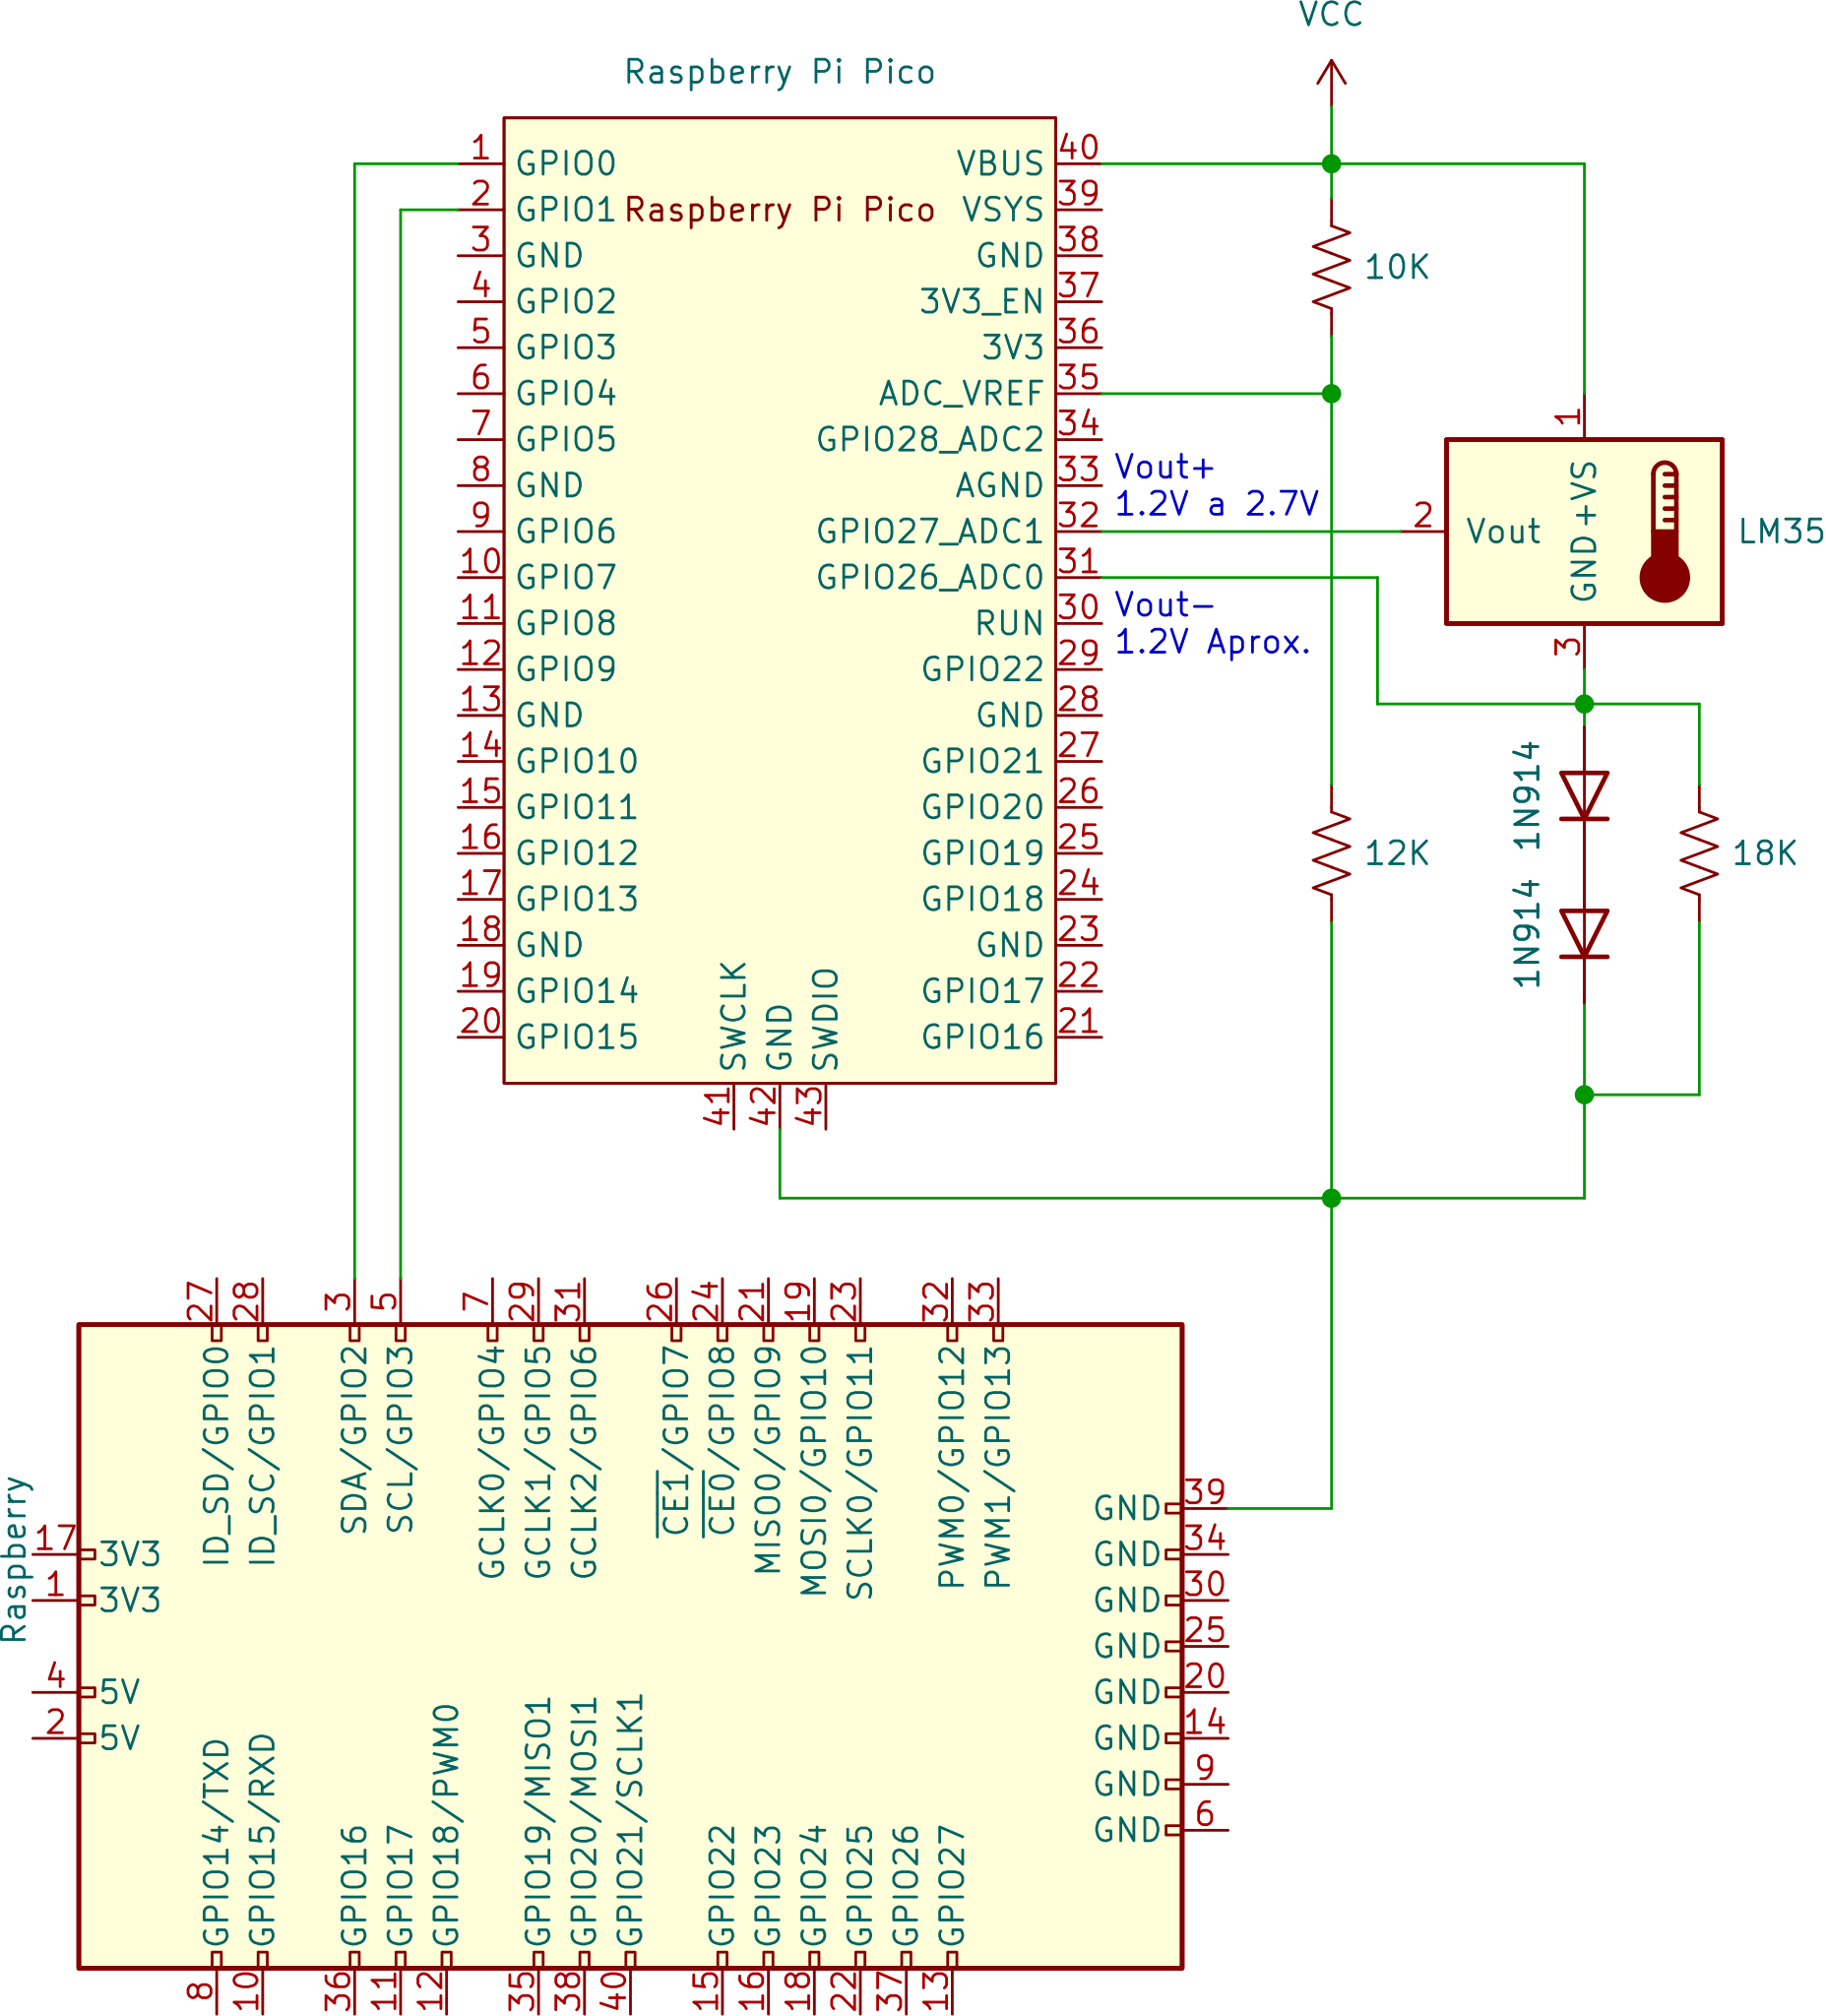
\includegraphics[width=\linewidth,height=7cm,keepaspectratio]{img/lm35-pico-pi.png}
	\caption{Circuito completo}
	\label{fig:circuit-full} % CHKTEX 24
\end{figure}
\end{minipage}%
\begin{minipage}{0.5\linewidth}
\begin{figure}[H]
	\centering
	\includegraphics[width=\linewidth,height=7cm,keepaspectratio]{img/pi-pico-i2c.png}
	\caption[Conexión de una Raspberry Pi con una Raspberry Pico via \IIC]{\centering Conexión mediante \IIC de una Raspberry Pi con una Raspberry Pico\footnotemark}%
	\label{fig:pi-pico-i2c} % CHKTEX 24
\end{figure}
\end{minipage}%
\footnotetext{Imagen obtenida de \url{https://python-academia.com/en/raspberry-pi-pico-slave/}}

\bigskip{}

Alambre primero el subcircuito formado por los dos diodos, el integrado LM35 y la resistencia de 18k$\Omega$.
Paso seguido, alimente el subcircuito y mida la diferencia de potencial existente entre V\textsubscript{OUT-} y \GND{}.
Utilice el valor medido en la fórmula $V_{ADC\_VREF} = 1.5V + V_{OUT-}$ para calcular los valores de las resistencias que se conectarán al pin ADC\_VREF del RP2040.

% \paragraph*{IMPORTANTE:}
\medskip
\begin{importantbox}{\large Importante}
	\begin{center}
		Asegúrese de que $V_{ADC\_VREF} \leq V_{OUT-}\Big|_{Temp=150^{o}C}$ para evitar quemar el RP2040.
	\end{center}
\end{importantbox}
\medskip

Continúe el alambrado del circuito.
Es conveniente colocar un capacitor de 0.1$\mu$F entre \VCC y \GND para rectificar el voltaje de entrada eliminar cualquier oscilación parásita que pudiere afectar el funcionamiento del LM35.
La presencia de este componente es opcional pero altamente recomendada.

\medskip
Tras alambrar el primer circuito realice el experimento prueba indicado en la \Cref{sec:step2}.
\medskip


A continuación conecte el bus \IIC entre la Raspberry Pi y el RP2040 como ilustran la \Cref{tbl:pi-pico-i2c} y la \Cref{fig:pi-pico-i2c}.


\begin{table}
	\centering
	\caption{Conexiones \IIC entre Raspberry Pi y un RP2040}
	\label{tbl:pi-pico-i2c} % CHKTEX 24
	\begin{tabularx}{0.7\linewidth}{cc rcl cc}
	\toprule
	\multicolumn{2}{c}{   Pin   } & \multicolumn{3}{c}{\multirow{2}{*}{Conexión}} & \multicolumn{2}{c}{  Pin  } \\
	\multicolumn{2}{c}{Raspberry} & \multicolumn{3}{c}{}                          & \multicolumn{2}{c}{RP2040 } \\
	\midrule
	       3 & (GPIO2)            & Raspberry Pi SDA & $\rightarrow$ & RP2040 SDA & GPIO0/SDA       &     1     \\
	       5 & (GPIO3)            & Raspberry Pi SCL & $\rightarrow$ & RP2040 SCL & GPIO1/SCL       &     2     \\
	       6 & (\GND)             & Raspberry Pi GND & $\rightarrow$ & RP2040 GND & \GND            &     3     \\
	\bottomrule
	\end{tabularx}
\end{table}


Esto es posible debido a que el RP2040 no cuenta con resistencias de acoplamiento a positivo o \emph{pull-up} integradas, mientras que los pines \IIC de la Raspberry Pi están conectados internamente a la línea de 3.3V mediante resistencias de 1.8k$\Omega$.
Por este motivo, tendrán que quitarse las resistencias de \emph{pull-up} a cualquier otro dispositivo esclavo que se conecte al bus \IIC de la Raspberry Pi.\footnote{Para más información sobre el papel de las resistencias de acoplamiento a positivo o \emph{pull-up} en un bus \IIC se puede consultar \url{http://dsscircuits.com/articles/effects-of-varying-i2c-pull-up-resistors} }
